\documentclass[sigconf, nonacm]{acmart}

\usepackage{booktabs}
\usepackage{graphicx}
\graphicspath{{../../figures/}}

\title{Query Scheduling Optimization in IVF-based Vector Search}

\author{Yujia Qian}
\email{yujia_qian@gsd.harvard.edu}
\affiliation{%
  \institution{Harvard University}
  \city{Cambridge}
  \state{Massachusetts}
  \country{USA}
}

\author{Xiangyu Guan}
\email{xiangyu_guan@gsd.harvard.edu}
\affiliation{%
  \institution{Harvard University}
  \city{Cambridge}
  \state{Massachusetts}
  \country{USA}
}

\begin{document}

\begin{abstract}
Vector search is a core component of modern AI systems, yet most
optimization efforts focus on index structure rather than query
execution. This paper investigates whether throughput can be improved by
batching concurrent queries over an IVF index to exploit overlap in the
inverted lists they probe, without modifying the index itself. We
compare two batching strategies, Batch(MV) and Batch(MM), against a
sequential baseline under random and clustered query workloads.
Experiments on SIFT1M confirm that batching consistently improves
throughput over sequential execution: Batch(MV) outperforms Sequential
by up to 19\% on random queries, while Batch(MM) achieves up to 40\%
gains on clustered queries, with all schedulers preserving identical
recall. The preferred scan mode shifts with the query distribution over
IVF clusters, and batch size further modulates the relative performance
between MV and MM.
A microbenchmark isolates the mechanism underlying these differences and
supports practical guidance on applying batch scheduling in IVF-based
vector search.
\end{abstract}

\keywords{vector search, IVF, batch scheduling, GEMM, query execution}

\maketitle

\section{Introduction}

Vector search is central to a wide range of AI applications, including
retrieval-augmented generation, semantic search, and recommendation
systems. Given a query vector, the system must efficiently return the
$k$ nearest neighbors from a large corpus of stored vectors. At scale,
such systems must sustain high query throughput while keeping tail
latency bounded.

The dominant approach to improving vector search performance is to
optimize the index structure. Hierarchical Navigable Small World graphs
(HNSW)~\cite{hnsw2020}, product quantization~\cite{pq2011}, and IVF
variants~\cite{faiss2021} have each offered significant gains in
recall-efficiency trade-offs. By contrast, the query execution
layer---how individual queries are dispatched and processed at
runtime---has received comparatively less attention.

This work takes the index as fixed and asks: \textbf{can throughput be
improved by reorganizing how concurrent queries are executed?}

We focus on IVF (Inverted File Index), which partitions the vector space
into clusters, each maintaining an inverted list of assigned vectors. To
answer a query, the engine identifies the nearest centroids and scans
the corresponding lists. Crucially, when multiple queries are processed
together, many of them probe overlapping lists. If the engine exploits
this overlap---loading each list once and computing distances for all
queries that need it---the total number of memory loads decreases
substantially.

Some recent systems have also focused on this batching strategy. Milvus
groups concurrent queries into cache-conscious blocks~\cite{milvus2021};
HQI batches queries over shared clusters for high-throughput vector
search~\cite{hqi2023}; Quake measures batching effects in the context of
adaptive indexing~\cite{quake2025}; and GPU-native IVF work uses
batching to expose GEMM-friendly computation and coalesced memory
access~\cite{ivfrabitq2025}. These systems demonstrate the value of
batching, but they do not isolate when GEMM-based list scanning should
replace per-query GEMV under a fixed index, nor how the query
distribution over IVF clusters and batch size govern that choice.

To study these conditions, we vary three aspects of the execution
setting. First, we compare random queries with clustered queries because
they induce different degrees of list overlap. Second, we compare two
scan modes: Batch(MV), which scans each list query by query, and
Batch(MM), which stacks queries sharing a list into a matrix-matrix
multiplication. Third, we vary batch size to determine how much
cross-query sharing is needed before batching and GEMM become effective.

This gap motivates four research questions:

\begin{itemize}
  \item \textbf{RQ1.} Does time-window batching improve throughput over
    sequential execution, under both random and clustered workloads?
  \item \textbf{RQ2.} How does scan mode choice (MV vs MM) affect
    performance under random versus clustered query distributions?
  \item \textbf{RQ3.} How does batch size affect the performance of
    batch schedulers?
  \item \textbf{RQ4.} What is the underlying mechanism that governs the
    relative performance of the two scan modes?
\end{itemize}

We organize the evaluation into three experiments: a main experiment
comparing all schedulers under fixed parameters, a batch-size sweep, and
a kernel microbenchmark. We find that batching can outperform
sequential execution, that the preferred scan mode changes with query
distribution and batch size, and that $L$---the number of queries
sharing each inverted list per batch---is the dominant variable behind
the MV--MM trade-off. These findings lead to practical guidelines for
choosing batch scheduling strategies under a fixed IVF index.

\section{Method}

\subsection{System Design}

\subsubsection{IVF Engine}

Our engine follows the IVF design from Faiss~\cite{faiss2021}: base
vectors are partitioned into 256 clusters via $k$-means, each cluster
maintaining an inverted list. We use Faiss for centroid training but
replace \texttt{index.search()} with a custom single-threaded implementation.
Faiss's search is a stateless black box that processes each query
independently, making cross-query optimizations invisible. Our engine
exposes centroid lookup and list scanning as separate interfaces, giving
the scheduler direct control over execution order and batch composition.

\subsubsection{Per-List Batch Scan}

When a batch of queries is dispatched together, multiple queries often
probe the same inverted list. The per-list batch scan exploits this by
iterating over inverted lists in list-major order: for each list,
distances are computed for all queries that probe it before moving to
the next. Each list is therefore loaded from memory exactly once per
batch, regardless of how many queries share it. This ``load once, serve
many'' principle mirrors cooperative scan techniques in column-store
databases~\cite{coopscans2007}.

We define \textbf{L} as the number of queries within a batch that probe
the same inverted list. Under sequential execution, $L = 1$ always.
Under time-window batching, $L$ grows with batch size and workload
query distribution over IVF clusters, and directly determines which scan
mode is more efficient.

\subsubsection{Scan Modes}

Two implementations of the per-list distance computation are provided,
differing in how they handle the $L$ queries sharing each list:

\textbf{Batch(MV).} Distances are computed for each of the $L$ queries
individually via a matrix-vector multiply (\texttt{vecs @ q}). Arithmetic
intensity is constant at $0.5$ FLOP/byte, independent of $L$.

\textbf{Batch(MM).} All $L$ queries are stacked into a query matrix and
distances are computed via a single matrix-matrix multiply
(\texttt{vecs @ Q.T}). Arithmetic intensity scales as $L/2$ FLOP/byte,
making MM increasingly efficient as $L$ grows. Prior work on GPU-native
IVF search has noted that batching queries enables GEMM-style execution
and coalesced memory access~\cite{ivfrabitq2025}; here we characterize
the crossover on CPU. GEMM carries non-trivial setup overhead at small
$L$, degrading performance relative to MV. The crossover point is
hardware-specific and is measured empirically in
Section~\ref{sec:microbench}.

\subsubsection{Schedulers}

Three configurations are evaluated (Table~\ref{tab:schedulers}).

\begin{table}
  \caption{Scheduler configurations.}
  \label{tab:schedulers}
  \begin{tabular}{lll}
    \toprule
    Scheduler  & Scan mode               & Batching policy \\
    \midrule
    Sequential & Single-query GEMV per list & None \\
    Batch(MV)  & Per-query GEMV per list & Time + batch size \\
    Batch(MM)  & GEMM per list           & Time + batch size \\
    \bottomrule
  \end{tabular}
\end{table}

Time-window batching accumulates arriving queries until either a time
limit $\Delta t$ elapses or a maximum batch size MaxBS is reached, then
dispatches all accumulated queries as a single batch. The dual trigger
bounds both waiting time at low load and memory pressure at high load.

\subsection{Experiment Design}

\subsubsection{Dataset}

All experiments use the SIFT1M benchmark~\cite{pq2011}: one million
128-dimensional SIFT descriptors, evaluated under L2 distance, with
10,000 held-out test queries and precomputed ground truth. All vectors
reside in memory; no disk I/O occurs during search.

\subsubsection{Workloads}

Query arrivals are simulated at a target rate of 2,000 QPS. Two
workloads are evaluated:

\textbf{Random.} All 10,000 SIFT test queries are used in their original
order. Each query probes a largely disjoint set of 8 inverted lists,
keeping $L$ small. This represents an adversarial case for batching:
list-reuse benefit is low, and any overhead from batch management
directly reduces throughput.

\textbf{Clustered.} Queries are filtered to those whose nearest centroid
falls among the 10 most-queried centroids, yielding 791 unique queries.
These are sorted by primary centroid and then tiled (round-robin
repetition) to reach 10,000 arrivals. Sorting by centroid ensures that
consecutive arrivals within each time window belong to the same cluster,
maximising $L$ per list per batch. All 791 queries are real SIFT test
vectors with valid ground truth, so Recall@10 is well-defined.

\subsubsection{Device}

All experiments are conducted on a MacBook Pro with an Apple M3 Pro chip
and 18\,GB unified memory. The engine runs single-threaded throughout to
isolate scheduling effects from multi-core parallelism.

\subsubsection{Experimental Protocol}

We use three experiments to answer the research questions introduced in
Section~1.

\textbf{Experiment 1 --- Main Experiment (RQ1, RQ2).} All three
schedulers are evaluated on both workloads under fixed parameters
($n_\text{clusters} = 256$, nprobe $= 8$, $k = 10$,
$\Delta t = 5$\,ms, MaxBS $= 128$) across 5 independent runs. Summary
statistics are reported as mean $\pm$ std; P99 latency is the median
across runs.

\textbf{Experiment 2 --- Batch Size Parameter Sweep (RQ3).} A grid
search is conducted once on both workloads:
\[
\begin{array}{ll}
\Delta t\ \mathrm{(ms)} & \in \{0.5, 1, 2, 5, 10, 20, 50\}, \\
\mathrm{MaxBS}          & \in \{32, 64, 128, 256\}.
\end{array}
\]

\textbf{Experiment 3 --- Microbenchmark (RQ4).} The MV and MM kernels
are evaluated in isolation on a synthetic inverted list across a range
of $L$ values, with 50 repetitions per point.

\section{Results}

We present results in three stages. First, the main experiment
demonstrates the core throughput claims under fixed scheduler
parameters. Second, the batch size parameter sweep shows how batch size
modulates the relative performance of MV and MM. Third, the
microbenchmark isolates $L$ as the underlying mechanism explaining both.

\subsection{Main Experiment}

All three schedulers are evaluated at fixed parameters
($\Delta t = 5$\,ms, MaxBS $= 128$) across 5 independent runs.

\subsubsection{Performance Overview}

Figure~\ref{fig:overview-qps} shows throughput across all three
schedulers under both workloads. The two lines cross between Batch(MV)
and Batch(MM): on the random workload, throughput peaks at Batch(MV)
then falls for MM; on the clustered workload, it rises monotonically
with MM taking the lead. This crossing is the central result of the
paper.

\begin{figure}
  \centering
  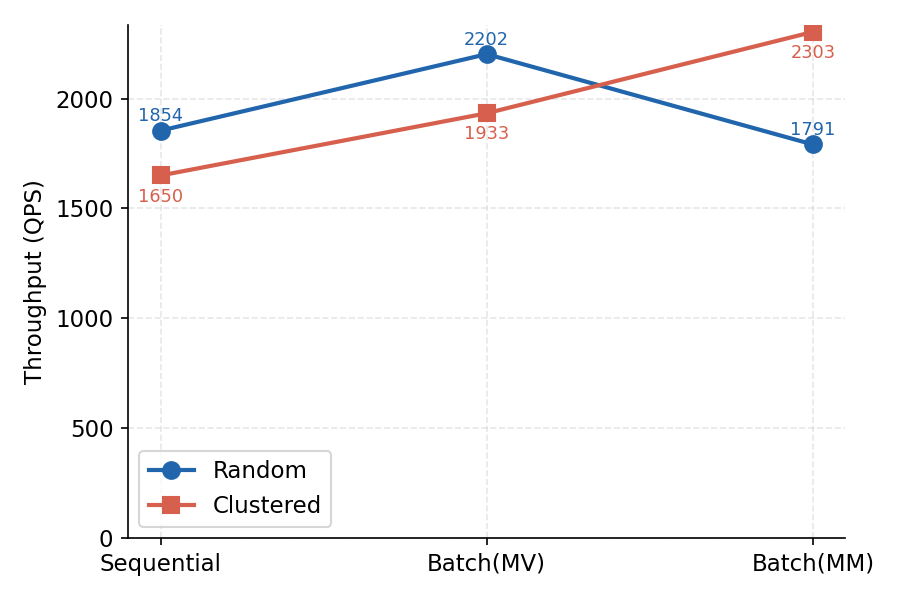
\includegraphics[width=\linewidth]{fig_overview_qps}
  \caption{Throughput (QPS) across schedulers for random and clustered
    workloads.}
  \label{fig:overview-qps}
\end{figure}

\begin{table}
  \caption{Throughput and Recall@10 (mean $\pm$ std, 5 runs).
    $\Delta t = 5$\,ms, MaxBS $= 128$.}
  \label{tab:main-results}
  \begin{tabular}{lrrrrr}
    \toprule
    Scheduler & QPS & Avg & P95 & P99 & Recall \\
              &     & (ms) & (ms) & (ms) & @10 \\
    \midrule
    \multicolumn{6}{l}{\textit{Random workload}} \\
    \midrule
    Sequential & $1{,}854 \pm 58$            & 0.54   & 0.74   & 0.81   & $0.957$ \\
    Batch(MV)  & $\mathbf{2{,}202 \pm 23}$   & 74.34  & 106.79 & 114.67 & $0.957$ \\
    Batch(MM)  & $1{,}791 \pm 87$            & 104.69 & 134.60 & 152.89 & $0.957$ \\
    \midrule
    \multicolumn{6}{l}{\textit{Clustered workload}} \\
    \midrule
    Sequential & $1{,}650 \pm 33$            & 0.61  & 0.78   & 0.88   & $0.981$ \\
    Batch(MV)  & $1{,}933 \pm 39$            & 96.19 & 127.30 & 139.06 & $0.981$ \\
    Batch(MM)  & $\mathbf{2{,}303 \pm 111}$  & 58.09 & 87.15  & 106.98 & $0.981$ \\
    \bottomrule
  \end{tabular}
\end{table}

Three findings stand out. First, batching can outperform Sequential:
Batch(MV) achieves $+19\%$ on random, and Batch(MM) achieves $+40\%$
on clustered. Second, the
relative ordering of MV and MM is reversed across workloads---MV leads
on random while MM leads on clustered. Third, these throughput gains
come with a latency trade-off from queueing: average latency rises from
${\sim}0.5$\,ms (Sequential) to 58--105\,ms for batch schedulers.
Recall@10 remains identical across all schedulers within each workload,
confirming that the gains arise from execution reorganization rather
than approximation.

\subsubsection{How Many Queries Share Each Inverted List ($L$)}

\begin{table}
  \caption{Mean per-list reuse metrics across 5 runs.}
  \label{tab:list-sharing}
  \begin{tabular}{lrrrr}
    \toprule
    Scheduler & Lists/query & $L$ mean & $L$ P50 & $L$ P95 \\
    \midrule
    \multicolumn{5}{l}{\textit{Random workload}} \\
    \midrule
    Sequential & 8.00 & 1.0  & 1 & 1  \\
    Batch(MV)  & 2.23 & 3.6  & 3 & 8  \\
    Batch(MM)  & 1.92 & 4.2  & 4 & 10 \\
    \midrule
    \multicolumn{5}{l}{\textit{Clustered workload}} \\
    \midrule
    Sequential & 8.00 & 1.0  & 1 & 1  \\
    Batch(MV)  & 0.55 & 14.6 & 5 & 64 \\
    Batch(MM)  & 0.65 & 12.4 & 5 & 52 \\
    \bottomrule
  \end{tabular}
\end{table}

Sequential always loads 8 lists per query with $L = 1$. On the random
workload, batching reduces unique list loads per query to 2.23
($3.6\times$ reduction), with mean $L = 3.6$--$4.2$. On the clustered
workload, this reduction reaches 0.55 lists per query, with mean
$L = 12.4$--$14.6$. The contrast in $L$ across the two workloads points
to the underlying mechanism distinguishing MV and MM
performance---addressed directly by the microbenchmark.

\subsection{Batch Size Parameter Sweep}

We sweep $\Delta t$ and MaxBS on both workloads to examine how batch
size affects the MV--MM trade-off. Four representative configurations
are selected per workload. The sequential baseline achieves 1,937 QPS
on random and 1,650 QPS on clustered. In Tables~\ref{tab:sweep-random}
and~\ref{tab:sweep-clustered}, $\Delta$QPS is computed as
$(\mathrm{MM}-\mathrm{MV})/\mathrm{MV}$.

\subsubsection{Random Workload}

\begin{table*}
  \caption{Selected ($\Delta t$, MaxBS) configurations --- random workload.}
  \label{tab:sweep-random}
  \begin{tabular}{rrrrrrr}
    \toprule
    $\Delta t$ (ms) & MaxBS & MV QPS & MM QPS & Mean $L$ (MV/MM) & MV Lat. (ms) & $\Delta$QPS (MM--MV) (\%) \\
    \midrule
    0.5               & 32               & 2,098          & 1,300          & 1.5/1.7 & 17.5  & $-38\%$ \\
    5                 & 64               & 2,230          & 1,446          & 2.5/2.5 & 42.3  & $-35\%$ \\
    \textbf{5}        & \textbf{128}     & \textbf{2,277} & \textbf{2,227} & \textbf{3.1/3.5} & \textbf{60.1} & $\mathbf{-2\%}$ \\
    20                & 256              & 2,322          & 2,562          & 7.3/5.8 & 160.8 & $+10\%$ \\
    \bottomrule
  \end{tabular}
\end{table*}

As $\Delta t$ and MaxBS grow, $L$ increases and MM's disadvantage
narrows and eventually reverses. At the smallest configuration
($\Delta t = 0.5$\,ms, MaxBS $= 32$), $L \approx 1.5$--$1.7$ places
both schedulers well below the hardware crossover, and MM's GEMM setup
overhead dominates ($-38\%$). At the main experiment parameters
($\Delta t = 5$\,ms, MaxBS $= 128$), $L$ rises to 3.1--3.5 and the gap
nearly closes ($-2\%$). At $\Delta t = 20$\,ms and MaxBS $= 256$,
$L$ reaches 5.8--7.3 and MM overtakes MV by 10\%. The throughput gains
come at a direct latency cost: MV average latency grows from 17.5\,ms
to 160.8\,ms, while the sequential baseline maintains ${\sim}0.5$\,ms.

\subsubsection{Clustered Workload}

\begin{table*}
  \caption{Selected ($\Delta t$, MaxBS) configurations --- clustered workload.}
  \label{tab:sweep-clustered}
  \begin{tabular}{rrrrrrr}
    \toprule
    $\Delta t$ (ms) & MaxBS & MV QPS & MM QPS & Mean $L$ (MV/MM) & MV Lat. (ms) & $\Delta$QPS (MM--MV) (\%) \\
    \midrule
    0.5               & 32               & 1,987          & 1,884          & 7.5/7.6   & 23.2  & $-5\%$  \\
    5                 & 64               & 1,934          & 2,156          & 11.1/11.0 & 48.7  & $+11\%$ \\
    \textbf{5}        & \textbf{128}     & \textbf{1,952} & \textbf{2,324} & \textbf{14.6/11.9} & \textbf{95.4} & $\mathbf{+19\%}$ \\
    20                & 256              & 1,948          & 2,424          & 17.8/17.3 & 192.3 & $+24\%$ \\
    \bottomrule
  \end{tabular}
\end{table*}

In contrast to the random workload, MM wins from small-to-medium batch
sizes because clustered queries share many lists, keeping
$L$ above the crossover even in small batches. At $\Delta t = 0.5$\,ms
and MaxBS $= 32$, $L \approx 7.5$--$7.6$ sits right at the hardware
crossover and MM barely loses ($-5\%$). As batch size grows, $L$ rises
well above the crossover and MM's advantage increases steadily to
$+24\%$.

Figure~\ref{fig:sweep} summarises the sweep results across both
workloads. The two trajectories---random rising from $-38\%$ and
clustered starting near zero---illustrate how the query distribution
over IVF clusters determines the operating regime of each scan mode.

\begin{figure}
  \centering
  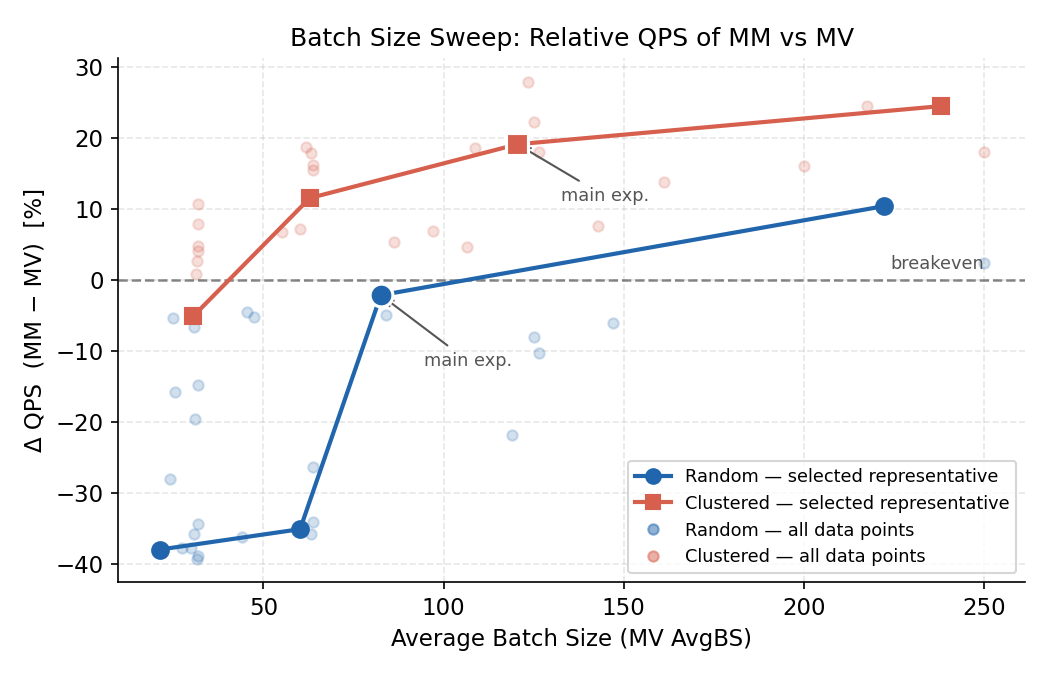
\includegraphics[width=\linewidth]{fig_sweep}
  \caption{Batch size sweep: relative QPS of MM vs MV across random and
    clustered workloads.}
  \label{fig:sweep}
\end{figure}

Figures~\ref{fig:latency-random} and~\ref{fig:latency-clustered} show
the latency cost of batching. On the random workload, both schedulers
incur substantially higher average latency than Sequential
(${\sim}0.5$\,ms); at small batches MM latency exceeds MV's due to GEMM
setup overhead, but at large batches MM's faster execution drains the
queue sooner. On the clustered workload, MM latency runs consistently
below MV because the high list-sharing rate gives MM a sustained
throughput advantage.

\begin{figure}
  \centering
  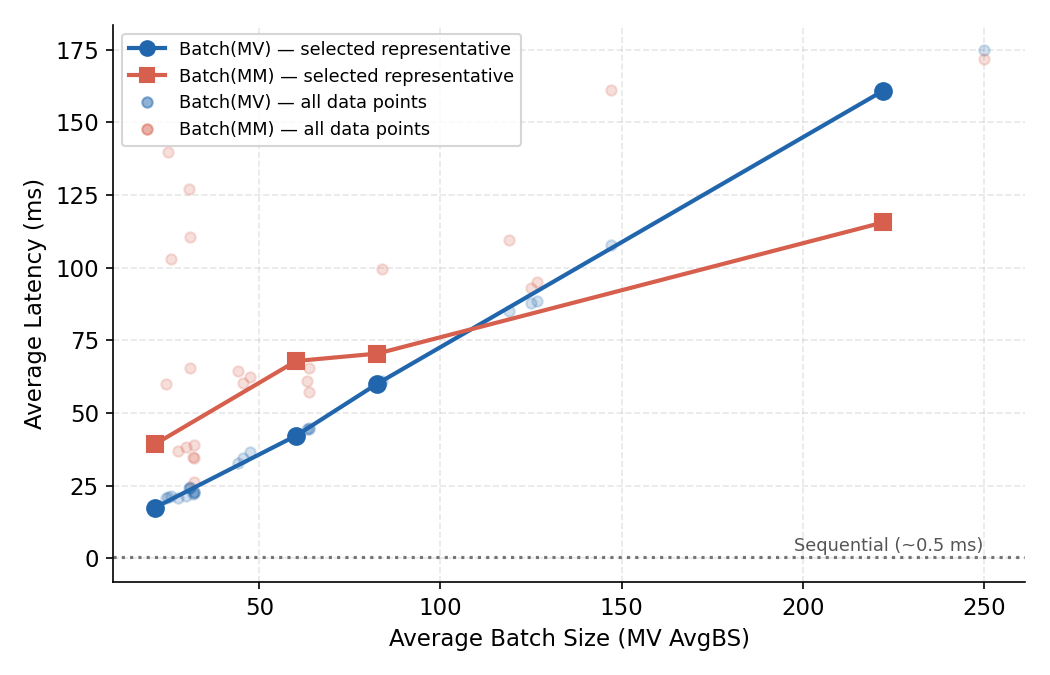
\includegraphics[width=\linewidth]{fig_latency}
  \caption{Average latency vs batch size on the random workload.}
  \label{fig:latency-random}
\end{figure}

\begin{figure}
  \centering
  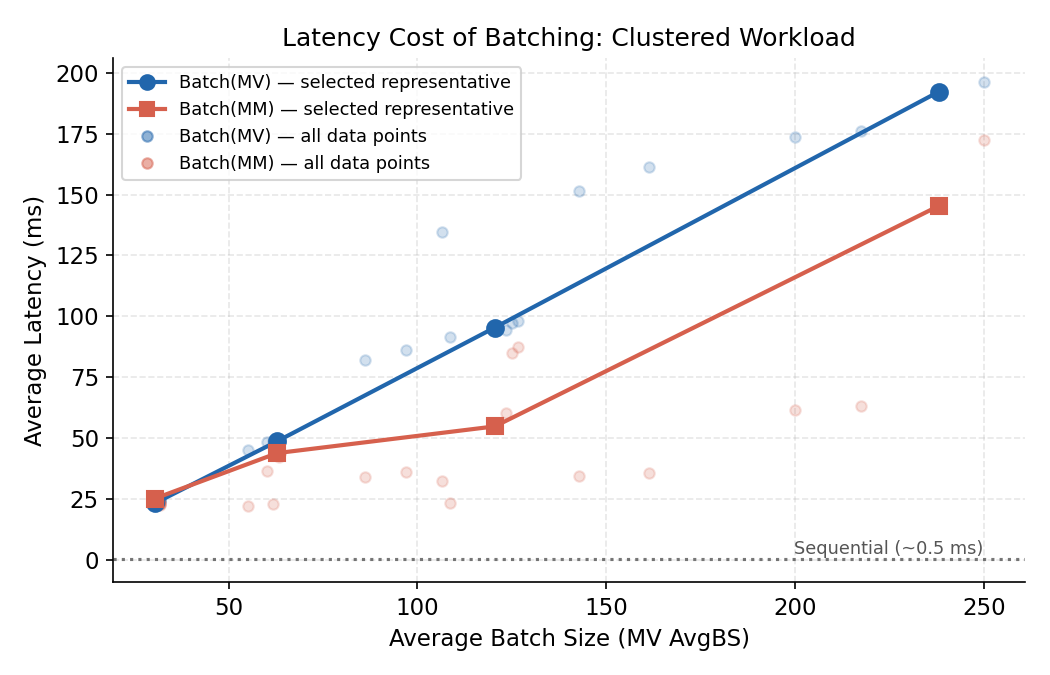
\includegraphics[width=\linewidth]{fig_latency_clustered}
  \caption{Average latency vs batch size on the clustered workload.}
  \label{fig:latency-clustered}
\end{figure}

\subsection{Microbenchmark}
\label{sec:microbench}

To isolate the effect of $L$ from scheduler dynamics, the MV and MM
kernels are benchmarked directly on a synthetic inverted list
($n = 4{,}000$ vectors, $d = 128$) for $L \in \{1, \ldots, 256\}$,
with 50 repetitions per point. Figure~\ref{fig:microbench} reports
kernel cost in ns/(query\,$\times$\,vector), so lower values indicate
higher throughput.

MV throughput is approximately constant across all values of $L$
(5.1--5.5\,ns/q$\cdot$v), as each query is processed independently. MM
throughput improves sharply with $L$, crossing the MV baseline at
$L = 8$ and reaching a $3.77\times$ speedup at $L = 256$. The crossover
corresponds to the point where GEMM arithmetic intensity
($L/2$ FLOP/byte) exceeds the GEMV baseline ($0.5$ FLOP/byte). In the
main experiment, mean $L \approx 3.6$--$4.2$ on random (below the
crossover) and mean $L \approx 12.4$--$14.6$ on clustered (above it),
fully accounting for the reversed MV--MM ordering observed in
Table~\ref{tab:main-results}.

\begin{figure}
  \centering
  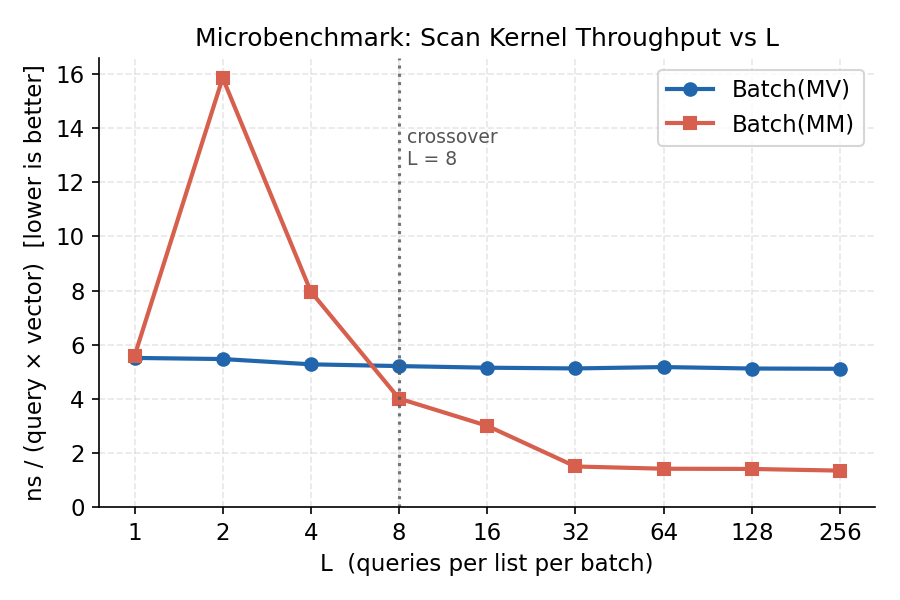
\includegraphics[width=\linewidth]{fig_microbench}
  \caption{Scan kernel throughput as a function of $L$.}
  \label{fig:microbench}
\end{figure}

\section{Discussion}

The experiments show that batching is useful for IVF query execution:
under the right workload and scan mode, batched execution can generate
higher QPS than sequential processing.

\textbf{Batching can improve throughput by reusing list work.}
The results indicate that time-window batching can improve throughput
without modifying the index or changing Recall@10. Its benefit comes
from reducing repeated list scans: unique list loads per query fall from
8 under Sequential to 2.23 on the random workload and 0.55 on the
clustered workload. This gain is not free, because time-window batching
introduces queueing and increases per-query latency; the saved scan work
therefore must outweigh the latency cost.

\textbf{The MV--MM choice is largely governed by $L$.}
Neither scan mode is uniformly best. Batch(MV) is stronger when each
inverted list is shared by only a few queries, because it avoids the
setup overhead of GEMM; Batch(MM) becomes stronger when enough queries
share the same list. The microbenchmark provides evidence for this
mechanism: MM overtakes MV around $L = 8$ on the experimental hardware,
near the point where GEMM arithmetic intensity exceeds the GEMV
baseline. Thus, in this setting, $L$---the number of queries within a
batch that probe the same inverted list---provides the most direct
explanation for scan-mode behavior.

\textbf{$L$ is shaped by batch size and query distribution.}
Larger batches place more queries in the same scheduling window, which
makes it more likely that multiple queries probe a common inverted list.
The query distribution over IVF clusters strengthens this effect by
determining whether co-batched queries actually touch the same lists.
This mechanism supports the batch-size sweep: increasing batch size and
using more concentrated query distributions can both raise $L$ and move
the system toward an MM-favorable regime.

\textbf{Practical Guideline.} These results suggest that a scheduler
should choose the scan mode from the $L$ induced by its batch size and
query distribution. A larger batch or a more concentrated query stream
can increase per-list sharing, but the scheduler should rely on the
observed $L$ rather than either factor alone. Low per-list sharing
favors Batch(MV), while high sharing favors Batch(MM). The crossover
point between the two should be measured for the target hardware and
workload.

\textbf{Limitations and Future Work.} The engine is deliberately
single-threaded to isolate scheduling effects; whether the observed gains
survive in a multi-core deployment remains an open question. An adaptive
strategy that switches between MV and MM per batch based on observed $L$
would eliminate the regression on random workloads while preserving
MM's advantage on clustered ones. All results are reported on SIFT1M;
validation on datasets with different dimensionalities or cluster
geometries would strengthen generalizability.

\bibliographystyle{ACM-Reference-Format}
\bibliography{references}

\end{document}
